\documentclass{CRPITStyle}


\usepackage[agsmcite]{harvard}
\usepackage[hang]{subfigure}
\usepackage{graphicx}


\pagestyle{empty}
\thispagestyle{empty}


\title{A Graphical Notation for Physical Database Modelling}
\author{Antonia Pillay \and Nigel Stanger}
\affiliation{Department of Information Science, \\
	University of Otago, \\
	PO Box 56, Dunedin, New Zealand \\
	Email:~\texttt{nstanger@infoscience.otago.ac.nz}}


\hyphenation{da-ta-base da-ta-ba-ses co-pies}


\begin{document}


\maketitle


\begin{abstract}
For database systems, physical level design is often as important as
conceptual level design, as it is the physical level that ultimately
determines the performance of a database system. It is therefore
somewhat surprising that there have been relatively few prior attempts
to devise an abstract graphical notation for physical level modelling.
Such a notation would provide database designers and administrators with
a means to consistently model the physical structure of new and existing
databases, thus enabling them to make more proactive and informed tuning
decisions, compared to the more typical situation where database
monitoring tools are used to identify and remedy performance problems in
a reactive and ad hoc manner. In this paper we propose an abstract
graphical notation for physical level database modelling, and compare it
with earlier work in this area.
\end{abstract}


\section{Introduction}

As with most information systems, the design and implementation of a
database goes through several phases, including conceptual, logical and
physical modelling \cite{BeDa-P-2003}. These three phases are of
particular interest, as they embody the progression from higher to lower
levels of abstraction \cite{Tsic-D-1978}. Conceptual models are
typically highly abstract, using techniques such as entity-relationship
modelling. Logical models represent the database structure in a form
that is closer to the physical representation, yet still abstracted
sufficiently to isolate applications from the physical representation
\cite{Codd-EF-1970}, and are expressed using formalisms such as the
relational model. A logical model for a database can be derived by
transforming the corresponding conceptual model.

Physical models represent the database structure in terms of the
internal physical storage implementation of a specific database
management system (DBMS) such as Oracle or DB2. A physical model for a
database can be derived by transforming the corresponding logical model
\cite{Bato-DS-1985,Conn-TM-2002}. Because of their low level of
abstraction, physical level database models have tended to not be
expressed using graphical notations, unlike models at higher levels of
abstraction.

Physical level modelling, however, is equally as important as, if not
\emph{more} important than the higher levels, because it is the physical
level that determines the performance of a database \cite{BeDa-P-2003}.
It is somewhat surprising that there have been relatively few attempts
to devise an abstract graphical notation for physical modelling, because
such a notation can provide several advantages
\cite{BeDa-P-1992-PDD,Conn-TM-2002,Tuft-ER-1997,Will-J-1992}:
\begin{itemize}

	\item it can reduce complexity and thus improve understandability;

	\item it can provide a more complete and integrated display of
	performance tuning techniques in a database;

	\item database developers can be more confident about the design
	decisions that they make for the performance of the database;

	\item potential database performance problem areas are more easily
	visualised using a graphical notation; and

	\item a specific methodology is developed and used, thus enabling
	developers to resolve physical performance issues more
	systematically.

\end{itemize}

Some of these benefits are embodied in modern database performance
monitoring tools, which provide higher-level visualisations of a
database's internals in order to easily identify and highlight
performance problems. Such tools, however, are primarily
\emph{monitoring} tools rather than \emph{design} tools. They may
therefore unintentionally encourage database administrators (DBAs) into
a reactive mode of continually ``tweaking'' the database to resolve
performance issues, rather than a proactive mode of anticipating and
designing for expected usage. It may also be difficult for a DBA using
such tools to gain a clear and comprehensive overview of all the tuning
techniques that are in use within a particular database
\cite{Core-MJ-1997-OracleDW}.

It could be argued that physical level structures vary so much from one
DBMS to another that it is futile to even consider a generic physical
modelling notation. However, examination of the major DBMS products in
use today reveals that they share many of the same physical tuning
techniques. The specific implementation of (for example) clustering may
vary in detail from platform to platform, but the feature is in concept
largely similar across all implementations. We provide a brief overview
of five such commonly used physical tuning techniques in
Section~\ref{sec-techniques}.

In this paper we propose an abstract graphical notation for physical
database modelling. In Section~\ref{sec-previous} we discuss two earlier
approaches upon which our work is partially based.
Section~\ref{sec-notation} introduces our notation, and
Section~\ref{sec-future} discusses possible future work. The paper
concludes in Section~\ref{sec-conclusion}.


\section{Common Physical Tuning Techniques}
\label{sec-techniques}

Database management is generally an I/O bound task, so the main
performance bottleneck in most database systems will be the performance
of tertiary storage devices such as disk drives. Retrieving data from a
hard disk is theoretically about five to six orders of magnitude slower
than retrieving data from RAM\footnote{On the order of milliseconds
(\(10^{-3}\)) for disk versus nanoseconds (\(10^{-9}\)) for RAM.}. The
aim of any physical tuning strategy must therefore be to minimise the
impact of slow tertiary storage, either by directly reducing the number
of physical disk accesses required, or by parallelising access to disk
in order to reduce contention.

These considerations have led to the development of five general
physical tuning techniques, which are implemented with slight variations
by most modern mainstream DBMS products:

\begin{description}

	\item[Indexes] reduce the number of physical disk accesses required
	to retrieve a specific record \cite{Roti-S-1996}, most typically by
	building a B+-tree \cite{Knut-DE-1997-Art} based on some key value
	within the data. Without any indexes, a DBMS often has little choice
	but to perform a sequential scan in order to locate a specific
	record. If we assume one disk access per database block, a
	sequential scan has average and worst case performance of \(K/2b\)
	and \((K - 1)/b\) disk accesses required, respectively, where \(K\)
	is the number of records and \(b\) is the number of records per
	database block. In contrast, a B+-tree has a worst case performance
	of \(\log_{n/2}(K)\) \cite{Silb-A-2002-4E}, where \(n\) is the
	number of key values per index node.

	\item[Hashing] is a method of quickly locating specific records by
	passing a key value to a \emph{hash function}. This function ideally
	returns a unique physical location of a hash bucket containing the
	requested physical record \cite{Pete-W-1957-hash}. Hashing schemes
	typically require only one or two physical disk accesses to retrieve
	a specific record, and perform best for exact key matches on very
	large tables. Hashing generally performs poorly for queries that
	require the retrieval of many records.

	\item[Clustering] minimises disk access by ensuring that related
	records (such as an order header and its associated order lines) are
	physically adjacent on disk \cite{Shas-DE-2003-tuning}. This usually
	means that related records will be stored in the same database
	block, and can thus be retrieved with a single disk access. The
	relationship between records is determined by a \emph{cluster key}
	comprising fields in common to both physical tables. Clustering can
	be expensive to maintain in a high update environment, because of
	the frequent ``reclustering'' required.

	\item[Partitioning] provides parallel access paths to data by
	physically splitting a table into disjoint parts (either vertically
	by columns or horizontally by rows) and placing them on separate
	disks \cite{Ceri-S-1982-partition}. This is particularly
	advantageous when multiple users wish to access different subsets of
	a set of records, because it provides a separate physical access
	path to each of the partitions. Partitioning can also reduce the
	number of disk accesses required, because there are fewer records to
	scan in each partition than if the table were not partitioned.

	\item[Replication] provides parallel access paths to data by making
	multiple copies of the same records and placing them on separate
	disks. This is particularly advantageous when multiple users need to
	access the same sets of records, but is more complex to manage due
	to the need to keep replicas synchronised.

\end{description}

These techniques are normally applied to different parts of a database
to achieve different effects. In order to choose an appropriate physical
tuning technique, the DBA must consider various factors that may benefit
only some users of the database, or may improve the performance of the
database as a whole. While most of the techniques can be combined to
varying degrees, simply applying all techniques is usually not optimal,
because each technique excels under different conditions. That is, what
are optimal conditions for one technique may be the exact opposite for
another, so the DBA needs to be able to model all available information
in order to develop an appropriate physical design.



\section{Prior Physical Modelling Techniques}
\label{sec-previous}

To achieve an effective physical design requires a large amount of
information, particularly with regard to the predicted or actual volume
and usage of data within the database \cite{BeDa-P-2003}. Incorporating
this information into a graphical model can provide a more concise and
clearer overview of the physical aspects of a database system. In this
section we briefly discuss two previous efforts at modelling such
information in a graphical manner.


\subsection{\emph{Agile Modeling}}

\citename{Ambl-SW-2003-ADT}
\citeyear{Ambl-SW-2003-ADT,Ambl-SW-2004-ObjPrimer3} proposed a physical
modelling notation based on the Unified Modelling Language (UML), as
part of a broader effort to develop a ``traditional'' style data
modelling profile for the UML. Ambler and others have argued the need
for such a profile for some time
\cite{Ambl-SW-1998-BOA,Naib-EJ-2001-UMLDD}.

Ambler's notation focuses on the physical modelling of relational
databases. The notation uses class boxes without stereotypes to
represent physical tables, while indexes are represented by class boxes
with the stereotype \verb|<<index>>|, as shown in
Figure~\ref{fig-Ambler}. There appear to be no stereotypes for other
physical tuning structures such as partitions, although these could be
easily incorporated.

\begin{figure*}[htb]
	\fbox{\parbox[b]{.99\linewidth}{%
		\vskip 0.5cm%
		\centerline{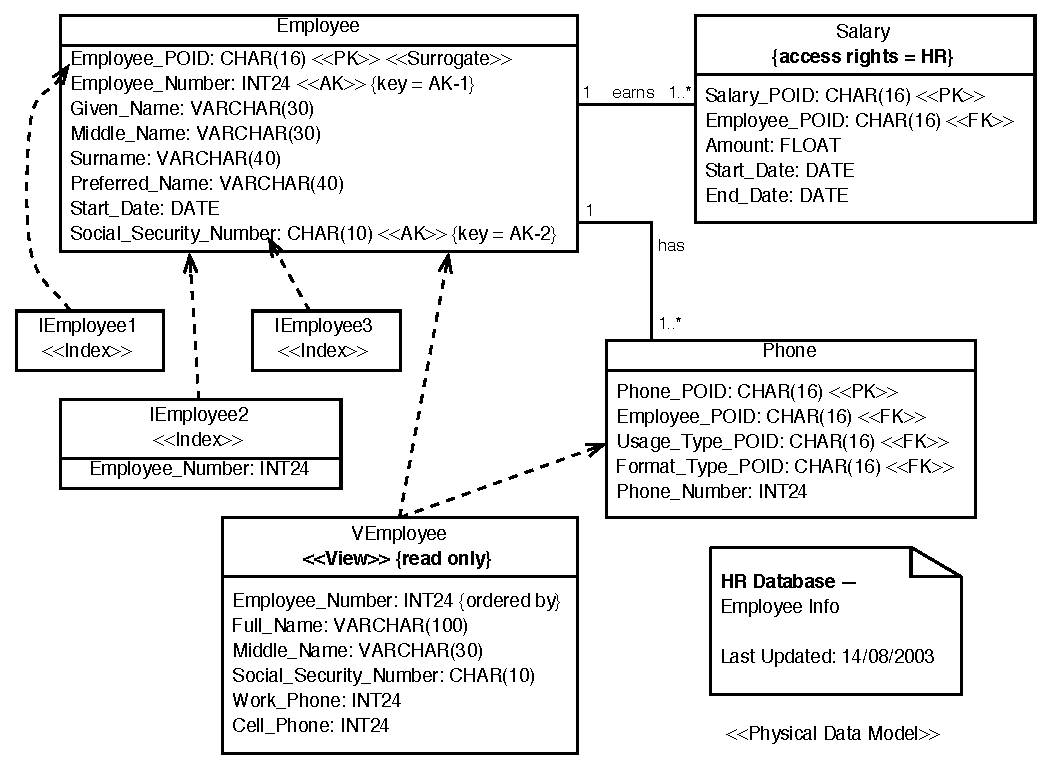
\includegraphics[scale=0.9]{Ambler}}%
		\vskip 0.5cm%
	}}
	\caption{Ambler's physical modelling notation \protect\citeaffixed{Ambl-SW-2003-ADT}{adapted from}}
	\label{fig-Ambler}
\end{figure*}

Ambler's approach suffers from two serious disadvantages. First, the
notation is very limited in the types of symbol used. All physical level
constructs are represented by almost identical class boxes, which in a
complex diagram could make distinguishing them difficult. This
limitation probably arises from the constraints on developing a new
notation within the existing UML framework.

Second, his approach appears to consistently confuse different levels of
abstraction: the same notations are used to represent not only physical
but also conceptual elements in the same diagram
\cite{Ambl-SW-2003-ADT}. This confusion is illustrated by the inclusion
of a view (a non-physical construct) in Figure~\ref{fig-Ambler}.

In summary, while Ambler's notation graphically models the physical
level of a database, the similarity of the graphical symbols and the
evident confusion between abstraction levels diminish its usefulness.


\subsection{\emph{Physical Design Using an Entity Model}}

\citeasnoun{BeDa-P-1992-PDD} proposed a method for analysing and
modelling the physical usage patterns of a database. In his method,
various physical aspects of a database are measured, such as the size
and expected growth rates of tables (volume analysis), the volatility of
tables, and the frequency of transactions (usage analysis). The data
obtained from these analyses are then used to annotate a logical level
entity-relationship diagram (ERD) of the database, producing what is
known as a \emph{composite usage map} (see
Figure~\ref{fig-Beynon-Davies} for an example).

Beynon-Davies' method provides a very good mechanism for representing
the usage statistics of a database in a coherent manner, but is rather
complex and time-consuming to undertake without some form of automation.
Our experience with teaching this method at undergraduate level shows
that even with a relatively small database, the designer can quickly
become overwhelmed by the sheer volume of usage data involved.

Furthermore, Beynon-Davies' method does not provide any way to model
specific tuning techniques---rather it summarises the information
required in order to decide which techniques should be applied.
Beynon-Davies' method is thus more a notation for summarising the
physical usage patterns of a database, rather than a notation for
physical modelling per se.


\section{A New Physical Notation}
\label{sec-notation}

Both of the notations discussed in the previous section are limited in
their ability to graphically model the physical level of a database.
Ambler's notation lacks clarity and is thus potentially confusing, while
Beynon-Davies' notation only summarises the physical usage patterns of a
database rather than providing an actual physical level model. We have
therefore adopted aspects from both approaches to devise a graphical
notation that enables database designers and administrators to
graphically model the common physical database tuning techniques
discussed in Section~\ref{sec-techniques}, thus gaining a clearer
picture of the tuning techniques applied to a database. The notation can
be used either to model the physical structures of an existing database
in preparation for further adjustment, or to design the physical
structures of a new database.

The symbols that we have adopted for this notation are shown in
Figure~\ref{fig-notation}. Some of these symbols are adapted from other
notations, while some we have created ourselves. The symbols have been
chosen to be intuitive and simple to draw, so as to produce diagrams
that are as clear and uncluttered as possible. Physical models may be
constructed using this notation either with or without a prior
Beynon-Davies style analysis.

\begin{figure*}[htb]
	\fbox{\parbox[b]{.99\linewidth}{%
		\vskip 0.5cm%
		\mbox{}%
		\hfill%
		\subfigure[Physical\newline{}table]{\label{fig-notation-table}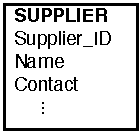
\includegraphics[scale=0.9]{notation-table}}%
		\hfill%
		\subfigure[Indexes]{\label{fig-notation-index}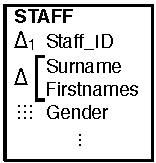
\includegraphics[scale=0.9]{notation-index}}%
		\hfill%
		\subfigure[Hashing]{\label{fig-notation-hash}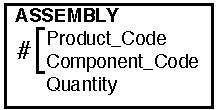
\includegraphics[scale=0.9]{notation-hash}}%
		\hfill%
		\subfigure[Replication]{\label{fig-notation-replica}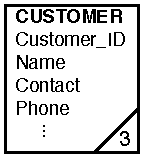
\includegraphics[scale=0.9]{notation-replica}}
		\hfill%
		\mbox{} \\%
		\mbox{}%
		\hfill%
		\subfigure[Clustering]{\label{fig-notation-cluster}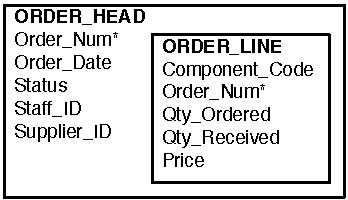
\includegraphics[scale=0.9]{notation-cluster}}%
		\hfill%
		\subfigure[Horizontal\newline{}partitioning]{\label{fig-notation-partition-h}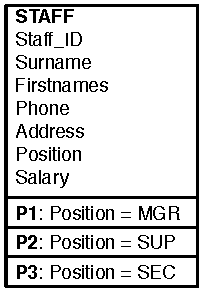
\includegraphics[scale=0.9]{notation-partition-h}}%
		\hfill%
		\subfigure[Vertical partitioning]{\label{fig-notation-partition-v}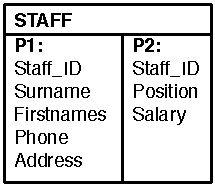
\includegraphics[scale=0.9]{notation-partition-v}}%
		\hfill%
		\mbox{}%
		\vskip 0.5cm%
	}}
	\caption{Symbols representing physical tuning techniques}
	\label{fig-notation}
\end{figure*}

A physical table is represented by a simple box, as shown in
Figure~\ref{fig-notation-table}. This is similar to most
entity-relationship modelling notations. The fields of the physical
table may be included with or without physical data types, as
appropriate. It could be argued that a different symbol should be used
to avoid confusion between, for example, physical tables and conceptual
entities. These constructs belong to different levels of abstraction,
however, so they should not both appear on the same diagram.
Consequently there is no real potential for confusion.

B-tree indexes are represented by the symbol ``\(\bigtriangleup\)''
(symbolising a tree structure) within a table, as shown in
Figure~\ref{fig-notation-index}. The index key is listed next to this
symbol. Composite keys are indicated by a grouping symbol, and a unique
index is indicated by a subscript ``1'', that is,
``\(\bigtriangleup_{1}\)''. Bitmap indexes \cite{Onei-PE-1987-bitmap}
and hashing are represented in a similar way, using the symbols
``\(\smash{\vdots\vdots\vdots}\)''\rule{0pt}{1.02\baselineskip} and
``\#'', respectively (see Figure~\ref{fig-notation-index}
and~\ref{fig-notation-hash}). Additional symbols could easily be defined
to cater for other types of index, such as R-trees.

Clustering is represented by nesting one table inside another, as shown
in Figure~\ref{fig-notation-cluster}
\citeaffixed{BeDa-P-1992-PDD}{adapted from}. The cluster key is
indicated by an asterisk (*) attached to the appropriate field(s).
Tables may be nested to as many levels as required in order to represent
more complex clustering schemes. This notation is intuitive, and clearly
indicates the field(s) on which the records are clustered. (Note that
the physical relationship connecting the clustered tables has been
omitted in Figure~\ref{fig-notation-cluster}.)

Partitioning is represented by splitting a table into either vertical or
horizontal partitions according to the style of partitioning, as shown
in Figure~\ref{fig-notation-partition-h} and
\ref{fig-notation-partition-v} \citeaffixed{Silb-A-2002-4E}{adapted
from}. Once again, the notation is intuitive, and allows the partition
names and definitions to be easily specified.

Replication is indicated by placing a diagonal bar across the lower
right corner of the table to be replicated, along with the total number
of replicas, as shown in Figure~\ref{fig-notation-replica}. This is
adapted from a similar notation used in data flow diagrams
\cite{Gane-C-1979}. This notation could also be used to indicate
replication of individual table partitions, for those DBMSs that permit
this combination. We considered an alternative symbol that looked like a
``stack'' of tables, on the basis that it might be useful to
differentiate between replicas. All the replicas are identical, however,
which diminishes the usefulness of such a symbol, and the symbol was
also more complex to draw.

Consider the entity-relationship diagram shown in Figure~\ref{fig-ERD},
which uses Martin notation \cite{Mart-J-1990-IE2} to depict a database
for a consumer electronics manufacturer (this was a case study used in
an undergraduate advanced database course). A corresponding
Beynon-Davies' composite usage map based on fourteen significant
transactions \cite{Pill-A-2005-DP} is shown in
Figure~\ref{fig-Beynon-Davies} (some details have been omitted for
clarity). The arrows represent physical access paths, while the number
attached to each access path indicates the estimated number of disk
accesses per hour along that path. The diagram clearly highlights some
potential performance problem areas in the database, for example:
\begin{itemize}

	\item There are many disk accesses per hour along the access paths
	between the \textsf{Sale\_head}/\textsf{Sale\_line} and (to a lesser
	extent) the \textsf{Order\_head}/\textsf{Order\_line} tables. Since
	records from each pair of tables will normally be accessed together,
	both pairs could perhaps be candidates for clustering, depending on
	the mix of update versus read operations.

	\item There appear to be multiple transactions accessing the
	\textsf{Staff} table along different access paths. This could imply
	a need for some form of partitioning.

	\item There is an extremely high access rate on the
	\textsf{Customer} table. Further investigation, however, reveals
	that this rate only occurs for a short period once per month, and
	that the transaction in question only requires read access.
	Replication of the \textsf{Customer} table could therefore be a
	suitable solution to ensure that this short, intense and
	intermittent transaction does not interfere with normal day-to-day
	transaction processing.
	
\end{itemize}


\begin{figure*}[htbp]
	\fbox{\parbox[b]{.99\linewidth}{%
		\vskip 0.5cm%
		\centerline{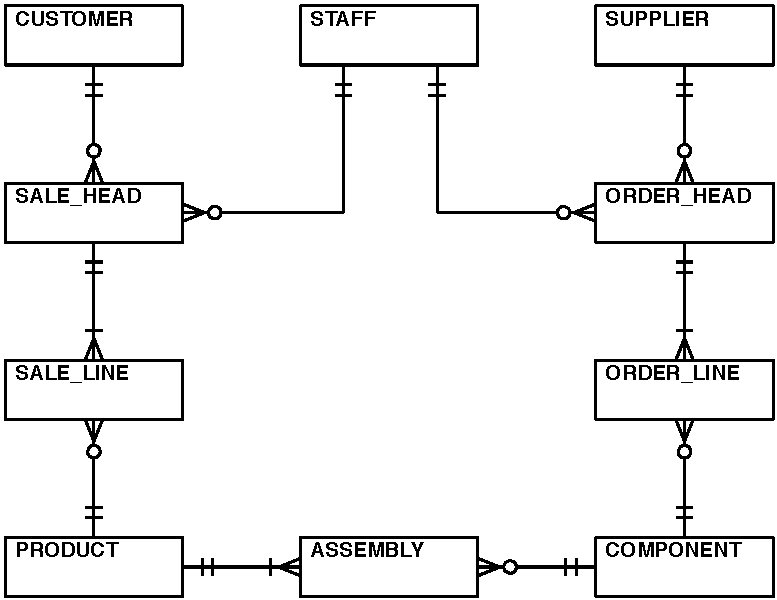
\includegraphics[scale=0.9]{ERD}}%
		\vskip 0.5cm%
	}}
	\caption{Logical level ERD of the example database}
	\label{fig-ERD}
\end{figure*}


\begin{figure*}[htbp]
	\fbox{\parbox[b]{.99\linewidth}{%
		\vskip 0.5cm%
		\centerline{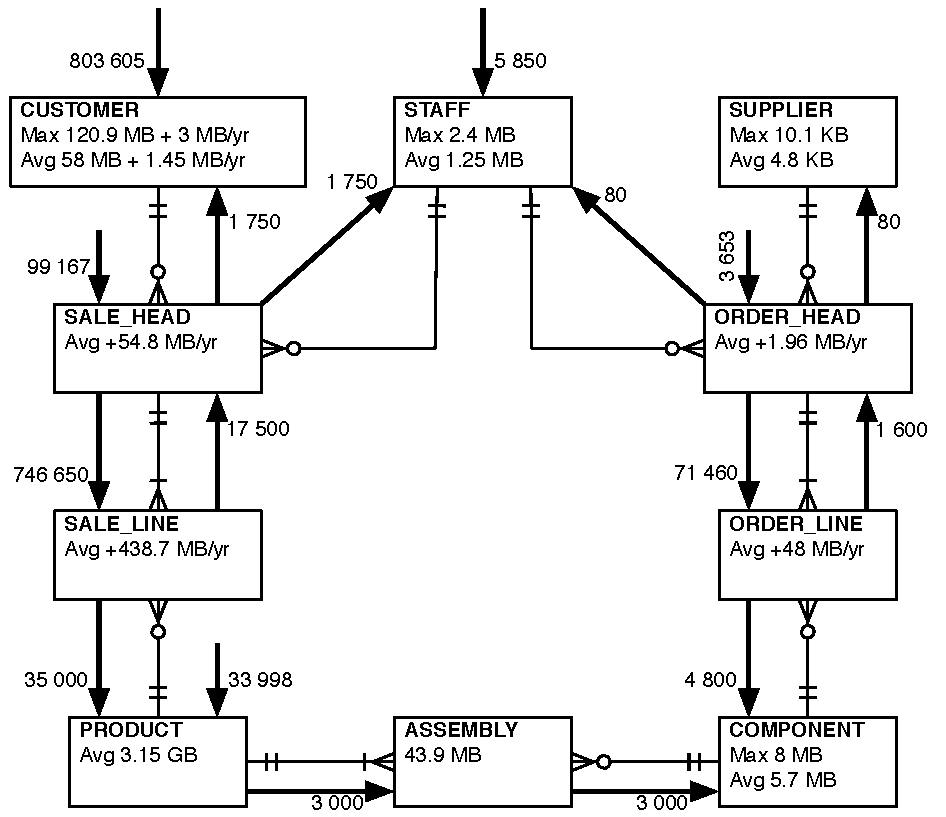
\includegraphics[scale=0.9]{Beynon-Davies}}%
		\vskip 0.5cm%
	}}
	\caption{Beynon-Davies composite usage map for the example database}
	\label{fig-Beynon-Davies}
\end{figure*}


The suggestions above can be represented as a physical model using our
modelling notation, as shown in Figure~\ref{fig-physical-model}. Note
that we have placed unique B-tree indexes on all primary keys as a
matter of course, as almost all DBMS products do this automatically, but
we have not included any other indexes. (In a real system, we would
often place indexes on commonly queried fields.) Looking at the diagram,
we can get a clear and concise picture of the techniques that have been
applied without being overwhelmed by irrelevant detail.


\begin{figure*}[htb]
	\fbox{\parbox[b]{.99\linewidth}{%
		\vskip 0.5cm%
		\centerline{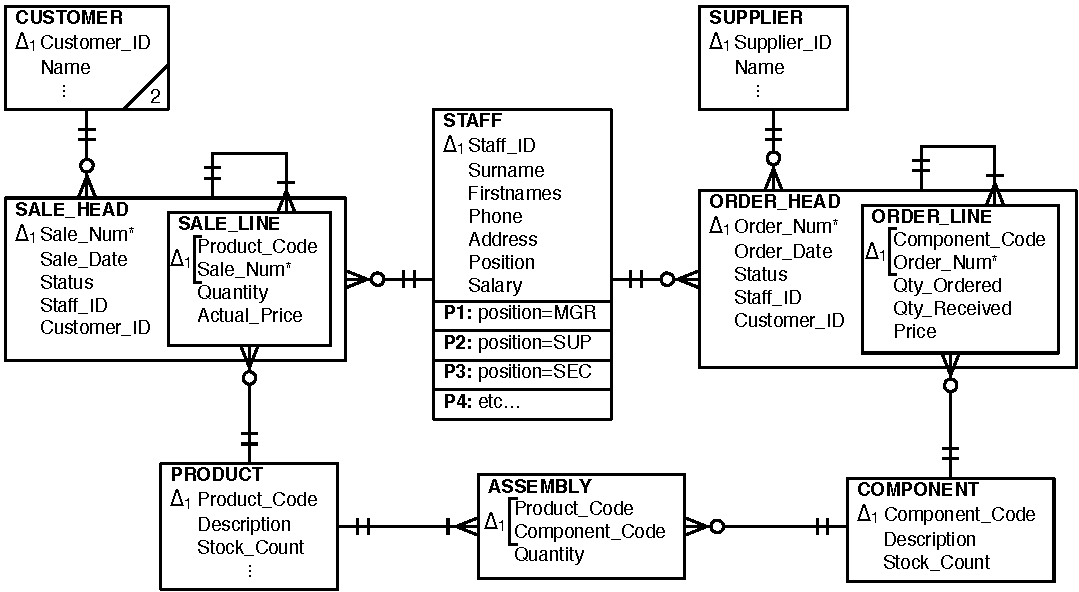
\includegraphics[scale=0.875]{Physical-Model}}%
		\vskip 0.5cm%
	}}
	\caption{Physical level model of the example database using the new notation}
	\label{fig-physical-model}
\end{figure*}


\section{Future Work}
\label{sec-future}

The current notation, while it covers the most common aspects of
physical modelling, is not complete and could be extended in various
ways, for example:
\begin{itemize}

	\item The current notation only caters for B-tree indexes, bitmap
	indexes and hashing. An obvious extension is to define symbols for
	other types of index, such as R-trees. We also plan to investigate
	symbols for index variants such as reverse-key and integrated
	indexes.
	
	\item Many DBMS products support partitioning of indexes in addition
	to tables. Our notation does not cater for this, but could possibly
	be modified so that indexes are modelled separately from their
	associated physical tables (similar to Ambler's notation). We would
	need to evaluate whether the benefits gained from such an extension
	would outweigh the additional diagrammatic complexity that it would
	introduce.
	
	\item There is currently no way to specify physical placement
	information such as which devices different partitions should be
	placed on.
	
	\item The clustering notation effectively assumes that there are at
	least two tables being clustered, but most DBMS products support
	single-table clusters, which in effect physically sort the contents
	of the table on the value of the cluster key. One solution would be
	to use a box symbol with a double border, that is,
	\fbox{\fbox{\mbox{}}}.
	
\end{itemize}

We are currently evaluating the efficacy of the notation with
undergraduate students in an advanced database course. We will then
compare this with using Beynon-Davies' method alone.

We also plan to develop tool support for our notation (currently the
diagrams must be produced manually). Given the similarity between our
notation and standard entity-relationship notations, it should not be
difficult to extend existing modelling tools to support the new
notation. It should also be possible to incorporate the notation into
more traditional database monitoring tools, which would provide DBAs
with a much clearer, in-context overview of the physical structure of
the database. Database activity could even be dynamically overlaid in
real-time on the physical model, thus revealing how effective different
tuning techniques are. Alternatively, the physical model could be used
with a simulation of projected database usage to determine how proposed
tuning techniques might affect database performance.



\section{Conclusion}
\label{sec-conclusion}

In this paper we have described a graphical notation for physical
database modelling, which enables database designers and administrators
to model the physical structure of new and existing databases in a more
abstract manner. This will enable them to make more proactive and
informed tuning decisions, compared to existing database monitoring
tools, which tend to encourage a more reactive and ad hoc approach to
database tuning. The notation uses simple and intuitive symbols to
represent common physical database structures and tuning techniques, and
can easily represent complex physical schemas.

The notation is currently being evaluated with undergraduate students in
an advanced database course; the results of this evaluation will be
compared with other physical modelling methods. We also plan to develop
tool support for the new notation.


\section*{Acknowledgements}

The authors would like to thank the students of \emph{INFO 321: Database
Systems} 2004 and 2005 for participating in the development and evaluation
of this new notation.


\bibliographystyle{agsm}

\bibliography{Physical_modelling}


\end{document}
